\subsection{1. Недетерминированные конечные автоматы (НКА). Различные варианты определений. Автоматные языки.}

\Def Алфавит $\Sigma$ — непустое конечное множество, элементы которого называются символами. При этом $\Sigma^*$ — множество слов, состоящее из всех слов $\Sigma$, $\varepsilon \in \Sigma^*$.

\Def Формальный язык $L$ — некоторое подмножество $\Sigma^*$.

\Def Недетерминированный конечный автомат (НКА) — кортеж $M = \langle Q, \Sigma, \Delta, q_0, F \rangle$:

\begin{enumerate}
    \item $Q$ — множество состояний, $Q$ — конечное множество, то есть $|Q| < \infty$;
    \item $\Sigma$ — алфавит;
    \item $\Delta \subset Q \times \Sigma^* \times Q$ — множество переходов \textit{(т.е. $\text{состояние}_{1} \xrightarrow{\text{слово}} \text{состояние}_{2}$)};
    \item $q_0 \in Q$ — стартовое состояние;
    \item $F \subset Q$ — множество завершающих состояний.
\end{enumerate}

\Def Конфигурация в автомате $\langle Q, \Sigma, \Delta, q_0, F \rangle$ — элемент $\langle q, w \rangle \in Q \times \Sigma^*$.

\Def Отношение $\vdash$ достижимости по $M$ — наименьшее рефлексивное транзитивное отношение над $Q \times \Sigma^*$, такое что:

\begin{enumerate}
    \item $\forall w \in \Sigma^* : (\langle q_1, w \rangle \rightarrow q_2) \in \Delta \Longrightarrow \langle q_1, w \rangle \vdash \langle q_2, \varepsilon \rangle$
    \item $\forall u, v \in \Sigma^* : \langle q_1, u \rangle \vdash \langle q_2, \varepsilon \rangle$, $\langle q_2, v \rangle \vdash \langle q_3, \varepsilon \rangle \Longrightarrow \langle q_1, uv \rangle \vdash \langle q_3, \varepsilon \rangle$
    \item $\forall u \in \Sigma^* : \langle q_1, u \rangle \vdash \langle q_2, \varepsilon \rangle \Longrightarrow \forall v \in \Sigma^* \langle q_1, uv \rangle \vdash \langle q_2, v \rangle$
\end{enumerate}

\begin{figure}[h]
    \hspace{-4ex} \begin{minipage}[h]{0.6\linewidth}
    \center{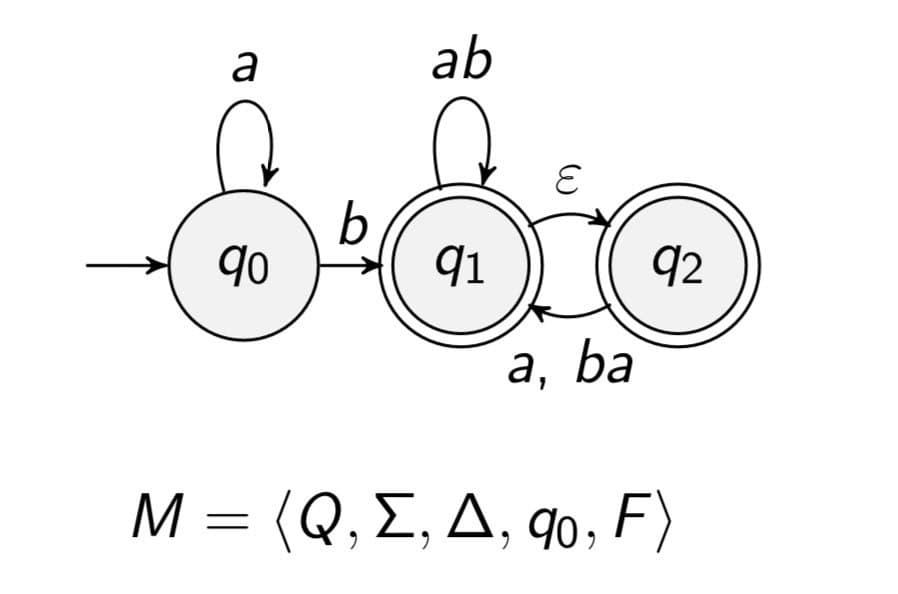
\includegraphics[width=0.6\linewidth]{1_1_1.jpg}}
    \end{minipage}
    \hfill
    \hspace{-4ex} \begin{minipage}[h]{0.5\linewidth}
    \Example Рассмотрим как автомат с картинки распознает слово $abab$:
    \newline $\langle q_0, abab \rangle \vdash \langle q_0, bab \rangle \vdash \langle q_1, ab \rangle \vdash \langle q_1, \varepsilon\rangle$ \\
    По транзитивности получаем: $\langle q_0, abab \rangle \vdash \langle q_1, \varepsilon\rangle$ \\
    \newline \textbf{Поясним переходы:} 
    \newline Первый и второй $\vdash$ работают по свойству 3, \newline а третий $\vdash$ работает по свойству 1.
    \end{minipage}
\end{figure}

\Def Для автомата $M = \langle Q, \Sigma, \Delta, q_0, F \rangle$ языком $L(M)$, задаваемым автоматом $M$, является множество $\{ w \in \Sigma^* \,\, | \,\, \exists q \in F : \langle q_0, w \rangle \vdash \langle q, \varepsilon \rangle \}$.

\Def Язык $L$ - автоматный, если существует такой НКА $M$, что $L = L (M)$.

\textbf{Утверждение об НКА с одним завершающим состоянием:} Для любого автоматного языка $L$ существует НКА $M' = \langle Q', \Sigma, \Delta', q_0', F' \rangle$, такой что $L(M') = L$, и $|F'| = 1$.

\textit{Идея доказательства:} добавим одно завершающее состояние $q_f$ на замену остальным и добавим $\varepsilon$-переходы из ''предыдущих'' завершающих состояний в новое. \newline \Vars$\vdash_i$ - достижимость за $i$ переходов

\Proof $L$ — автоматный язык, значит, существует НКА $M = \langle Q, \Sigma, \Delta, q_0, F \rangle$, такой что $L (M) = L$. Введём $M' = \langle Q \cup \{ q_f \}, \Sigma, \Delta', q_0, \{ q_f \} \rangle$, где $\Delta' = \Delta \cup \{ \langle q, \varepsilon \rangle \mapsto q_f \,\,|\,\, q \in F \}$. Далее нужно доказать, что $L (M) = L(M')$.

Докажем, что $L(M) \subset L (M')$. По определению из того, что $w \in L (M)$, следует, что существует состояние $q \in F$, что $\langle q_0, w \rangle \vdash \langle q, \varepsilon \rangle$. В автомате $M'$ есть переход $\langle q, \varepsilon \rangle \mapsto q_f \Longrightarrow \langle q, \varepsilon \rangle \vdash \langle q_f, \varepsilon \rangle$. Так как $\langle q_0, w \rangle \vdash \langle q, \varepsilon \rangle \vdash \langle q_f, \varepsilon \rangle$, то $w \in L (M')$.
\begin{figure}[h]
    \hspace{-4ex} \begin{minipage}[h]{1\linewidth}
    \center{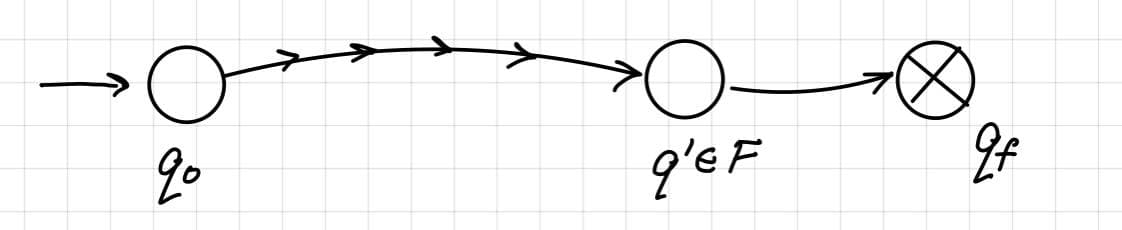
\includegraphics[width=0.6\linewidth]{1_1_2.jpg}}
    \end{minipage}
    \hspace{-4ex}
\end{figure}

Докажем, что $L (M) \supset L (M')$. Из того, что $w \in L (M')$, следует, что $\langle q_0, w \rangle \vdash \langle q_f, \varepsilon \rangle$. Но так как в $q_f$ можно добраться только по $\varepsilon$-переходу, то существует состояние $q'$, что $\langle q_0, w \rangle \vdash \langle q', \varepsilon \rangle \vdash_1 \langle q_f, \varepsilon \rangle \Longrightarrow q' \in F$. А в автомате $M$ $\langle q_0, w \rangle \vdash \langle q', \varepsilon \rangle$. Значит, $w \in L(M)$. \EndProof

\textbf{Утверждение об НКА с не более однобуквенными переходами:} Для любого автоматного языка $L$ существует НКА $M = \langle Q, \Sigma, \Delta, q_0, F \rangle$, такой что $L = L(M)$ и $\forall (\langle q_1, w \rangle \mapsto q_2) \in \Delta$ $|w| \leqslant 1$

\begin{center}
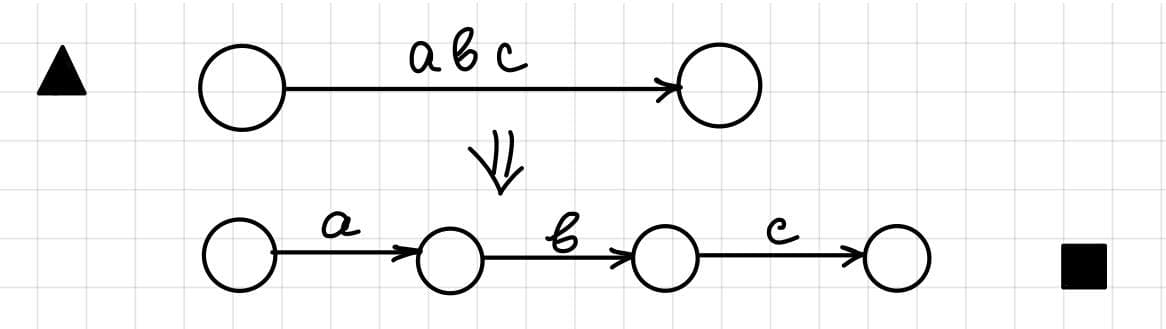
\includegraphics[width=0.6\linewidth]{1_1_3.jpg}
\end{center}

\textbf{Теорема об НКА с однобуквенными переходами:} Для любого НКА $M = \langle Q, \Sigma, \Delta, q_0, F \rangle$ существует НКА $M' = \langle Q, \Sigma, \Delta', q_0, F' \rangle$, такой что $L (M) = L (M')$ и:
$$\forall (\langle q_1, w \rangle \rightarrow q_2) \in \Delta \quad |w| = 1$$
\Proof Обозначим множество вершин, достижимых из $q$ по $w$ как $\Delta (q, w) = \{ q' | \langle q, w \rangle \vdash \langle q', \varepsilon \rangle \}$. Считаем, что в любом переходе $|w| \leqslant 1$. Введём следующие множества:

\begin{center}
    $F' := \{ q \,\,|\,\, \Delta (q, \varepsilon) \cap F \neq \varnothing \}$
    
    $\Delta' = \{ \langle q_1, a \rangle \rightarrow q_2 \,\, |\,\, \exists q_3 \in \Delta (q_1, \varepsilon) : \langle q_3, a \rangle \rightarrow q_2 \}$
\end{center}

Докажем, что $L(M') = L(M)$

Пусть $w\in L(M')$. Тогда $\exists q' \in F' : \langle q_0, w \rangle \vdash_{M'} \langle q', \varepsilon \rangle$. 

Тогда $\exists q \in F : \Delta(q',\varepsilon) = q \Longrightarrow \langle q', \varepsilon \rangle \vdash_{M} \langle q, \varepsilon \rangle$.

Рассмотрим $w = w_1 w_2 \dots w_n$. Тогда верно следующее:
$$
\forall m \; \exists q_m' \; : \; \angles{q_{m-1}', w_m} \rightarrow q_m' \in \Delta' \;\; (q_m' := q') \quad (1)
$$
%m-1
Значит, $\exists q_{m} \; : \; \Delta(q_{m-1}', \varepsilon) = q_{m}, \; \angles{q_{m}, w_m} \rightarrow q_m'$ \ и \ $\angles{q_{m-1}', w_{m}}\vdash_M \angles{q_m', \varepsilon} \quad (2)$

Из (1) и (2) следует, что 
$$
\angles{q_0', w_1\ldots w_m}\vdash_M\angles{q_1', w_2\ldots w_m}\vdash_M\angles{q_2', w_3\ldots w_m}\ldots\vdash_M\angles{q_m', w_m}\vdash_M\angles{q, \varepsilon}
$$
Следовательно, $w\in L(M)$.
% Докажем следующее утверждение:

% \begin{center}
%     $\exists q \in F : \langle q_0, w \rangle \vdash_M \langle q, \varepsilon \rangle \Longleftrightarrow \exists q' \in F' : \langle q_0, w \rangle \vdash_{M'} \langle q', \varepsilon \rangle$
% \end{center}

% Пусть $w = w_1 w_2 \dots w_n$, $w \in L(M') \Longrightarrow \exists q' \in F' : \langle q_0, w \rangle \vdash_{M'} \langle q, \varepsilon \rangle$. Из однобуквенности всех переходов:

% \begin{center}
%     $\exists q_1, \dots, q_n : \langle q_0, w_1 \dots w_n \rangle \vdash_{M'} \langle q_1, w_2 \dots w_n \rangle \vdash_{M'} \dots \vdash_{M'} \langle q_{n - 1}, w_n \rangle \vdash_{M'} \langle q_n, \varepsilon \rangle$
    
%     $q_n \in F' \Longrightarrow \exists q'' \in F : q'' \in \Delta (q_n, \varepsilon) \Longrightarrow \langle q_n, \varepsilon \rangle \vdash_M \langle q'', \varepsilon \rangle$ \qquad $(1)$
    
%     $\brackets{\langle q_{k - 1}, w_k \rangle \overset{M'}{\rightarrow} q_k} \Longrightarrow \exists \overset{\sim}{q_k} \in Q$
    
%     $\overset{\sim}{q_k} = \Delta \brackets{q_{k - 1}, \varepsilon}$
    
%     $\langle \overset{\sim}{q_k}, w_k \rangle \rightarrow q_k \in \Delta$
    
%     $\langle q_{k - 1}, \varepsilon \rangle \vdash_M \langle \overset{\sim}{q_k}, \varepsilon \rangle$
    
%     $\langle q_{k - 1}, w_k \rangle \vdash_M \langle q_k, \varepsilon \rangle$ $\brackets{2}$
% \end{center}

% \noindent Из $\brackets{1}$ и $\brackets{2}$ следует, что существует $q'' \in F$, такой что $\langle q_0, w_1 \dots w_n \rangle \overset{\brackets{2}}{\vdash_M} \langle q_1, w_2 \dots w_k \rangle \overset{\brackets{2}}{\vdash_M} \dots \overset{\brackets{2}}{\vdash_M} \langle q_n, \varepsilon \rangle \overset{\brackets{1}}{\vdash_M} \langle q'', \varepsilon \rangle$, откуда $w = w_1 \dots w_n \in L \brackets{M}$. 

\par В обратную сторону: $w \in L(M) \Rightarrow \exists q \in F: \: \langle q_0, w \rangle \vdash_M \langle q, \varepsilon \rangle$. Пусть $w=w_1w_2$ (для больших n аналогично). Тогда есть цепь \begin{itemize}
    \item $\langle q_0, w_1w_2 \rangle \vdash_M \langle q_1', w_1w_2 \rangle$
    \item $\langle q_1', w_1w_2 \rangle \vdash_{M,1} \langle q_1, w_2 \rangle$ (читаем символ $w_1$)
    \item $\langle q_1, w_2 \rangle \vdash_M \langle q_2', w_2 \rangle$
    \item $\langle q_2', w_2 \rangle \vdash_{M,1} \langle q_2, \varepsilon \rangle$ (читаем символ $w_2$)
    \item $\langle q_2, \varepsilon \rangle \vdash_M \langle q, \varepsilon \rangle$
\end{itemize}
\par Получаем, что $\Delta(q_0, \varepsilon)=q_1', \: \langle q_1', w_1 \rangle \rightarrow q_1 \Rightarrow \langle q_0, w_1 \rangle \rightarrow q_1 \in \Delta'$.

\par Аналогично $\langle q_1, w_2 \rangle \rightarrow q_2 \in \Delta'$. Так как $\Delta(q_2, \varepsilon)=q \in F \Rightarrow q_2 \in F'$.
\par Тогда $\langle q_0, w_1w_2 \rangle \vdash_{M'} \langle q_1, w_2 \rangle \vdash_{M'} \langle q_2, \varepsilon \rangle$ и $w=w_1w_2 \in L(M')$
\EndProof

